% !TEX root = main.tex
\chapter{Topology Hiding Computation}\label{chap:THC}
In this chapter, we describe a few results in the study of Topology Hiding Computation, exploring different cryptographic assumptions, models for communication, and kinds of adversaries.
First, we show that we can realize all current standard-assumption THC constructions by via Learning-With-Errors (see \cite{C:Regev06}). This is because all of the current constructions rely on a type of encryption called Privately-Key-Commutative-Randomizable encryption (\PKCR), described in more detail in Section \ref{sec:pkcr-desc}.
Then, we will explore what an asynchronous model for THC could look like. We show that, unfortunately, all standard notions of asynchronous models give the adversary too much power to achieve even topology-hiding broadcast.
Overall, this result shows how strong of a primitive THC is, and how difficult it is to achieve it.

This chapter is based off of sections from both \cite{LLMMMT18} and \cite{LLMMMT20}.

\section{Overview}
Overview stuff..
%TODO: overview

\subsection{Results and Techniques}
results and stuff..
%TODO: 

\section{Preliminaries for Topology Hiding Computation}\label{sec:thc-prelim}
% !TEX root = ../main.tex
In this section, we will go over the preliminaries for \THC. This will include a primer on previous protocols and the tools necessary for them. 

\subsection{Graphs and Random Walks}
In an undirected graph $G = (V,E)$ we denote by $\nbh{\party_i}$ the neighborhood of $\party_i \in V$. The $k$-neighborhood of a party $\party_i \in V$ is the set of all parties in $V$ within distance $k$ to $\party_i$.

The following lemma from \cite{C:AkaLaVMor17} states that in an undirected connected graph $G$, the probability that a random walk of length $8|V|^3 \tau$ covers $G$ is at least $1- \frac{1}{2^\tau}$. 

\begin{lemma}[\cite{C:AkaLaVMor17}]\label{lem:randomWalkCover}
	Let $G = (V,E)$ be an undirected connected graph. Further let $\mathcal{W}(u,\tau)$ be a random variable whose value is the set of nodes covered by a random walk starting from $u$ and taking $8|V|^3 \tau$  steps. We have
	\begin{equation*}
	\Pr_\mathcal{W}[\mathcal{W}(u,\tau) = V] \ge 1- \frac{1}{2^\tau}.
	\end{equation*} 
\end{lemma}

\subsection{Random Walk Protocol from \texorpdfstring{\cite{C:AkaLaVMor17}}{[ALM17a]}}\label{sec:RandomWalks}

The most efficient protocol for THC is from \cite{C:AkaLaVMor17}, and techniques (e.g. random walks) are the only known techniques for achieving \THC~in a passive adversarial setting in polynomial communication and rounds under standard assumptions. We present a summary of it here so that it is easy to understand why \PKCR~is important and how current methods break down in an asynchronous setting.

We recall that the random walk protocol achieves security against static passive corruptions. To achieve broadcast, the protocol actually computes an OR.  Every party has an input bit: the sender inputs the broadcast bit and all other parties use 0 as input bit. Computing the OR of all those bits is thus equivalent to broadcasting the sender's message.

First, we will explain a simplified version of the protocol that is unfortunately not sound, but this gets the principal across. Each node will take its bit, encrypt it under a public key and forward it to a random neighbor. The neighbor OR's its own bit, adds a fresh public key layer, and it randomly chooses the next step in the walk that the message takes, choosing a random neighbor to forward the bit. Eventually, after about $O(\secparam n^3)$ steps, the random walk of every message will visit every node in the graph, and therefore, every message will contain the OR of all bits in the network. Now we start the backwards phase, reversing the walk and peeling off layers of encryption.

This scheme is not sound because seeing where the random walks are coming from reveals information about the graph! So, we need to disguise that information. We will do so by using correlated random walks, and will have a walk running down each direction of each edge at each step (the number of walks is then 2$\times$ number of edges). The walks are correlated, but still random. This way, at each step, each node just sees encrypted messages all under new and different keys from each of its neighbors. So, intuitively, there is no way for a node to tell anything about where a walk came from.

In more detail, and to demonstrate security, consider a single node $v$ with $d$ neighbors. During the forward phase at step $t$, $v$ gets $d$ incoming messages --- one from each of its neighbors
homomorphically OR's its bit to each, computes $d$ fresh public keys, adding a layer to each, and finally computes a random permutation $\pi_t$ on its neighbors, forwarding the message it got from neighbor $i$ to neighbor $\pi_t(i)$ and so on. During the backwards phase, node $v$ removes the public key layers it added during the corresponding forward round, and then reverses the permutation, sending the message it got from neighbor $j$ to neighbor $\pi_t^{-1}(j)$. Because all messages are encrypted under semantically secure encryption, $v$ cannot tell whether it has received a 0 or 1 from any of its neighbors, and because all of its neighbors are layering their own fresh public keys onto the messages, there is no way for $v$ to tell where that message came from or if it had seen it before. Intuitively, this gives us soundness (see \cite{C:AkaLaVMor17} for details).

Now, this protocol is also correct: every walk will, with all but negligible probability, visit every node in the network, and therefore every message will, with all but negligible probability, contain an encryption of the OR of all bits in the graph by the end of the forward phase. The backward phase then takes that message at the end of the walk, and reverses the walk exactly, popping off the public key layer that was added at each step. By the end of the backward phase, the node that started the walk gets the decryption of the message: the OR of all bits in the graph. Because all of the walks succeed, and every node started a walk, every node gets the correct output bit as desired.


\subsection{OR-Homomorphic PKCR Encryption Scheme}\label{sec:pkcr-desc}
In \cite{C:AkaLaVMor17} and \cite{EC:AkaMor17}, protocols require a public key encryption scheme with additional properties, called \emph{Privately Key Commutative and Rerandomizable encryption}.
We assume that the message space is bits. Then, a PKCR encryption scheme should be: (1) privately key commutative and (2) homomorphic with respect to the OR operation. We formally define these properties below.
\footnote{PKCR encryption was introduced in \cite{EC:AkaMor17,C:AkaLaVMor17}, where it had three additional properties: key commutativity, homomorphism and rerandomization, hence, it was called Privately Key Commutative and \emph{Rerandomizable} encryption. However, rerandomization is actually implied by the strengthened notion of homomorphism. Therefore, we decided to not include the property, but keep the name.}

Let $\PK$, $\SK$ and $\cC$ denote the public key, secret key and ciphertext spaces. As any public key encryption scheme, a PKCR scheme contains the algorithms $\keygen:\{0,1\}^* \to \PK \times \SK$, $\enc:\{0,1\} \times \PK \to \cC$ and $\dec:\cC \times \SK \to \{0,1\}$ for key generation, encryption and decryption respectively (where $\keygen$ takes as input the security parameter).

For a public-key $\pk$ and a message $m$, we denote the encryption of $m$ under $\pk$ by $\encrypted{m}{\pk}$. Furthermore, for $k$ messages $m_1,\dots,m_k$, we denote by $\encrypted{m_1,\dots,m_k}{\pk}$ a vector, containing the $k$ encryptions of messages $m_i$ under the same key $\pk$.

For an algorithm $\algorithm{A}(\cdot)$, we write $\algorithm{A}(\cdot \ ;U^*)$ whenever the randomness used in $\algorithm{A}(\cdot)$ should be made explicit and comes from a uniform distribution. By $\approx_c$ we denote that two distribution ensembles are computationally indistinguishable.

\subsubsection{Privately Key-Commutative}
We require $\PK$ to form a commutative group under the operation $\keymul$. So, given any $\pk_1, \pk_2 \in \PK$, we can efficiently compute $\pk_3 = \pk_1 \keymul \pk_2 \in \PK$ and for every $\pk$, there exists an inverse denoted $\pk^{-1}$. 
This $\pk^{-1}$ must be efficiently computable given the secret key corresponding to $\pk$.

This group must interact well with ciphertexts; there exists a pair of efficiently computable algorithms $\AddLayer : \cC \times \SK \to \cC$ and $\DelLayer : \cC \times \SK \to \cC$ such that
\begin{itemize}
	\item For every public key pair $\pk_1, \pk_2 \in \PK$ with corresponding secret keys $\sk_1$ and $\sk_2$, message $m \in \cM$, and ciphertext $c = [m]_{\pk_1}$,
	\[\AddLayer(c, \sk_2) = [m]_{\pk_1 \keymul \pk_2}.\]
	\item For every public key pair $\pk_1, \pk_2 \in \PK$ with corresponding secret keys $\sk_1$ and $\sk_2$, message $m \in \cM$, and ciphertext $c = [m]_{\pk_1}$,
	\[\DelLayer(c, \sk_2) = [m]_{\pk_1 \keymul \pk_2^{-1}}.\]
\end{itemize}
Notice that we need the secret key to perform these operations, hence the property is called \emph{privately} key-commutative.

\subsubsection{OR-Homomorphic}
We also require the encryption scheme to be OR-ho\-mo\-mor\-phic, but in such a way that parties cannot tell how many 1's or 0's were OR'd (or who OR'd them). 
We need an efficiently-evaluatable homomorphic-OR algorithm, $\homOr : \cC \times \cC \to \cC$, to satisfy the following: for every two messages $m, m' \in \{0,1\}$ and every two ciphertexts $c, c' \in \cC$ such that $\dec(c, \sk) = m$ and $\dec(c, \sk) = m'$,
\begin{gather*}
\left\{ (m,m', c,c', \pk, \enc(m \lor m', \pk; U^*)) \right\} \\
\approx_c \\
\left\{ (m,m', c,c', \pk, \homOr(c, c', \pk; U^*)) \right\}\\
\end{gather*}
Note that this is a stronger definition for homomorphism than usual; usually we only require correctness, not computational indistinguishability.

In \cite{C:HMTZ16}, \cite{EC:AkaMor17} and \cite{C:AkaLaVMor17}, the authors discuss how to get this kind of homomorphic OR under the DDH assumption, and later \cite{EPRINT:AkaLaVMor17} show how to get it with the QR assumption. For more details on other kinds of homomorphic cryptosystems that can be compiled into OR-homomorphic cryptosystems, see \cite{EPRINT:AkaLaVMor17}.

In this thesis we show how to instantiate a PKCR encryption scheme under the LWE assumption (see Section \ref{sec:lwe-pkcr}).

%------------ PKCR ------------%
\section{Privately Key-Commutative Randomizable\texorpdfstring{\\}
	Encryption (PKCR) from LWE}
% !TEX root = ../main.tex

In this section we show how to get a PKCR encryption scheme from the LWE assumption.
Basis of our PKCR scheme is the public-key crypto-system proposed in \cite{C:Regev06}. Let us briefly recall the public-key crypto-system:

\paragraph{LWE PKE scheme \cite{C:Regev06}}
Let $\kappa$ be the security parameter of the cryptosystem. The cryptosystem is parameterized by two integers $m$, $q$ and a probability distribution $\chi$ on $\mathbb{Z}_q$. To guarantee security and correctness of the encryption scheme, one can choose $q \ge 2$ to be some prime number between $\kappa^2$ and $2\kappa^2$, and let $m = (1+\epsilon)(\kappa+1)\log q$ for some arbitrary constant $\epsilon > 0$. The distribution $\chi$ is a discrete gaussian distribution with standard deviation $\alpha(\kappa) \coloneqq \frac{1}{\sqrt{\kappa}log^2\kappa}$.
%We need that the public keys form a group $\langle \mathcal{PK}, \cdot \rangle$. Given public keys $\pk = A\cdot \sk + \mathbf{e}$, $\pk' = A \cdot \sk' + \mathbf{e}'$, we define the combined public key as $\pk \cdot \pk' \coloneqq \pk + \pk'$.

\begin{description}
	\item[Key Generation:]
	
	\emph{Setup}: For $i = 1,\dots,m$, choose $m$ vectors $\mathbf{a}_1,\dots,\mathbf{a}_m \in \mathbb{Z}_q^{\kappa}$ independently from the uniform distribution. Let us denote $A \in \mathbb{Z}_{q}^{m\times \kappa}$ the matrix that contains the vectors $\mathbf{a}_i$ as rows.
	
	\emph{Secret Key}: Choose $\mathbf{s} \in \mathbb{Z}_{q}^{\kappa}$ uniformly at random. The secret key is $\sk = \mathbf{s}$.
	
	\emph{Public Key}: Choose the error coefficients $e_1,\dots,e_m \in \mathbb{Z}_q$ independently according to $\chi$. The public key is given by the vectors $b_i = \langle \mathbf{a}_i,\sk \rangle + e_i$. In matrix notation, $\pk = A\cdot \sk + \mathbf{e}$.
	
	\item[Encryption:] To encrypt a bit $b$, we choose uniformly at random $\mathbf{x} \in \{0,1\}^{m}$. The ciphertext is $c = (\mathbf{x}^{\intercal} A, \mathbf{x}^{\intercal} \pk + b\frac{q}{2})$.
	
	\item[Decryption:] Given a ciphertext $c = (c_1,c_2)$, the decryption of $c$ is $0$ if $c_2 - c_1\cdot \mathsf{sk}$ is closer to $0$ than to $\lfloor \frac{q}{2} \rfloor$ modulo $q$. Otherwise, the decryption is $1$.
	%Correctness: $c_2 - c_1\cdot \mathsf{sk} = x^{\top} \cdot e + b\frac{q}{2} \approx b\frac{q}{2}$. 
\end{description}

To extend this scheme to a PKCR scheme, we need to provide algorithms to rerandomize ciphertexts, to add and remove layers of encryption, and to homomorphically compute the OR. To obtain the OR-homomorphic property, it is enough to provide a XOR-Homomorphic PKCR encryption scheme, as was shown in~\cite{EPRINT:AkaLaVMor17}.

\paragraph{Extension to PKCR} 
We now extend the above PKE scheme to satisfy the requirements of PKCR (cf. Section~\ref{sec:pkcr-desc}). 
For this we show how to rerandomize ciphertexts, how add and remove layers of encryption, and finally how to homomorphically compute XOR.

\begin{description}
	
	\item[Rerandomization:] We note that a ciphertext can be rerandomized, which is done by homomorphically adding an encryption of $0$. The algorithm $\lweRand$ takes as input a cipertext and the corresponding public key, as well as a (random) vector $\mathbf{x} \in \{0,1\}^{m}$.
	
	\begin{algobox}{$\lweRand(c = (c_1,c_2),\pk,\mathbf{x})$}
		\begin{algorithmic}
			\State \Return $(c_1 + \mathbf{x}^{\intercal} A,c_2 + \mathbf{x}^{\intercal}\pk)$.
		\end{algorithmic}
	\end{algobox}
	
	\item[Adding and Deleting Layers of Encryption:] Given an encryption of a bit $b$ under the public key $\pk = A\cdot \sk + \mathbf{e}$, and a secret key $\sk'$ with corresponding public key $\pk' = A \cdot \sk' + \mathbf{e}'$, one can add a layer of encryption, i.e. obtain a ciphertext under the public key $\pk \cdot \pk' \coloneqq A \cdot (\sk + \sk') + \mathbf{e} + \mathbf{e}'$. Also, one can delete a layer of encryption.
	
	\begin{algobox}{$\lweAdd(c = (c_1,c_2),\sk)$}
		\begin{algorithmic}
			\State \Return $(c_1,c_1\cdot \sk + c_2)$
		\end{algorithmic}
	\end{algobox}
	
	\begin{algobox}{$\lweDel(c = (c_1,c_2),\sk)$}
		\begin{algorithmic}
			\State \Return $(c_1,c_2 - c_1\cdot \sk)$
		\end{algorithmic}
	\end{algobox}
	
	\textbf{Error Analysis}
	Every time we add a layer, the error increases. Hence, we need to ensure that the error does not increase too much. After $l$ steps, the error in the public key is $\pk_{0\dots l} = \sum_{i = 0}^{l} \mathbf{e}_i$, where $\mathbf{e}_i$ is the error added in each step.
	
	The error in the ciphertext is $c_{0\dots l} = \sum_{i = 0}^{l} \mathbf{x}_{i} \sum_{j=0}^{i} \mathbf{e}_j$, where the $\mathbf{x}_{i}$ is the chosen randomness in each step. Since $\mathbf{x}_i \in \{0,1\}^{m}$, the error in the ciphertext can be bounded by $m \cdot \max_{i}\{\abs{\mathbf{e}_i}_{\infty}\} \cdot l^2$, which is quadratic in the number of steps.
	
	\item[Homomorphic XOR:] A PKCR encryption scheme requires a slightly stronger version of homomorphism. In particular, homomorphic operation includes the rerandomization of the ciphertexts. Hence, the algorithm $\lweHxor$ also calls $\lweRand$. The inputs to $\lweHxor$ are two ciphertexts encrypted under the same public key and the corresponding public key.
	%Given two encryptions $c,c'$ of two bits $b,b'$ respectively, one can compute an encryption of $b \oplus b'$ by adding the ciphertexts. %Note that this operation works always
	
	\begin{algobox}{$\lweHxor(c = (c_1,c_2),c' = (c_1',c_2'),\pk)$}
		\begin{algorithmic}
			\State Set $c'' = (c_1 + c_1', c_2 + c_2')$.
			\State Choose $\mathbf{x} \in \{0,1\}^{m}$ uniformly at random.
			\State \Return $\lweRand(c'',\pk,\mathbf{x})$
		\end{algorithmic}
	\end{algobox}
\end{description}\label{sec:lwe-pkcr}

%------------ Asynch Models ------------%
\section{Barriers to Asynchronous Topology Hiding}\label{sec:impossible}
% !TEX root = ../main.tex

All previous results for \THC~are in the \emph{fully synchronous} model, where a protocol proceeds in rounds. This model makes
two assumptions: first, the parties have access to synchronized clocks, and 
second, every message is guaranteed to be delivered within one round.
While the first assumption is reasonable in practice, as nowadays computers 
usually stay synchronized with milliseconds of variation, the second assumption 
makes protocols inherently impractical.
In practice, the first assumption appears reasonable, since nowadays computers 
usually stay synchronized with milliseconds of variation. On the 
other hand, the second assumption makes protocols inherently impractical. 
This is because the running time of 
a protocol is always counted in the number of rounds, and the round length must be chosen based on the most pessimistic bound 
on the message delivery time.
For concreteness, consider a network where most of the time messages are delivered within milliseconds, but one of 
the connections, once in a while, may slow down to a couple of hours. In this 
case, a round would have to take a couple of hours.



%TODO: asynch section
\subsection{Standard Asynchronous Models}
% !TEX root = ../main.tex

The common models for asynchronous communication 
\cite{STOC:BenCanGol93,FOCS:Canetti01} consider a worst-case scenario and give 
the adversary the power to schedule the messages.

In more depth, the model of \cite{STOC:BenCanGol93} has the protocol communication described as a sequence of steps, where only one party is active each step. The catch is that a scheduler gets to adversarially decide on the order of the steps. The scheduler is `oblivious,' meaning it does not know what messages are being sent at each step, but does know who is sending a message to whom.

The UC-model, detailed in \cite{FOCS:Canetti01}, provides a more general approach to asynchronous multiparty (distributed) protocols. In this model, the adversary gets direct access to all channels connecting parties. He can both read all messages sent along these paths \emph{and} determine when messages are finally delivered.

Notice that in both of these models, the ability to schedule messages means the adversary automatically learns which parties 
are communicating. As a consequence, it is unavoidable that the adversary 
learns the topology of the communication graph, which we want to hide. A first attempt to rectify this problem would be to use a separate adversary that schedules messages from the adversary that corrupts parties: a scheduler and a corrupter, where topology-hiding would be guaranteed as long as the corrupter does not learn anything beyond the local structure of the communication graph. However, if the scheduler is also adversarial, he can signal to the corrupt parties what kind of graph the network is. For example, if there is a triangle in the graph, the scheduler would know, and could delay the first message along \emph{all} channels by 3 seconds (and would not delay messages otherwise). An adversary would then immediately be able to distinguish between a communication graph with a triangle and one without.
\subsection{THC is Impossible with Adversarial Delays}
% !TEX root = ../main.tex

Since the previous models inherently do not work in our setting, a natural definition would be to give the adversary control over 
scheduling on channels from only his corrupted parties. However, we will show that any reasonable 
model in which the adversary has the ability to delay messages for an 
unbounded 
amount of time allows him to learn something about the topology of the graph.
In essence, a very long delay from a party behaves almost like an abort, and 
an 
adversary can exploit this much like a fail-stop adversary in the 
impossibility 
result of \cite{MOR15}. We formally prove this in a very weak 
adversarial model.

First, note that if we have bounded delays, we can always use a synchronous protocol, starting the next round after waiting the maximum delay. So, in order for this model to be interesting, we must assume the adversary has unbounded delays.
In order to be as general as possible, we prove this with the weakest model we can while still giving the adversary some control over its delays: the adversary can only add delay to messages leaving corrupt nodes.

Our proof will follow the structure of \cite{MOR15}, using a similar game-based definition and even using the same adversarially-chosen graphs (see figure \ref{fig:imp}). Our game is straightforward. The adversary gives the challenger two graphs and a set of corrupt nodes so that the corrupt neighborhoods are identical when there is no adversarially added delay. The challenger then chooses one of those graphs at random, runs the protocol, and gives the views of all corrupt nodes to the adversary. The adversary wins if she can tell which graph was used. In \cite{MOR15}, the adversary would choose a round to failstop one of its corrupt parties. In our model, the adversary will instead choose a time (clock-tick) to add what we call a long-delay (which is just a very long delay on sending that and all subsequent messages). The adversary will be able to detect the delay based on when the protocol ends: if the delay was early in the protocol, the protocol takes longer to finish for all parties, and if it was late, the protocol will still finish quickly for most parties.

This impossibility result translates to an impossibility in the simulation-based setting since a secure protocol for the simulation-based setting would imply a secure protocol for the game-based setting.

Since delays cannot depend on the adversary without leaking topology, delays 
are an inherent property of the given network, much like in real life. As 
stated before, we give each edge a delay distribution, and the delays of 
messages traveling along that edge are sampled from this distribution. This 
allows us to model real-life networks where the adversary cannot tamper with 
the network connections. For example, on the Internet, delays between two 
directly connected nodes depend on their distance and the reliability of their 
connection.

\begin{figure}
	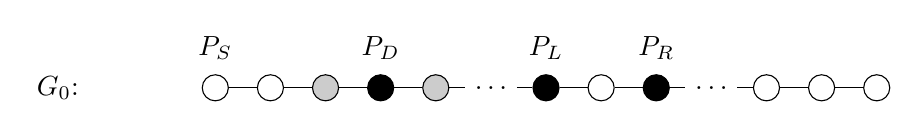
\begin{tikzpicture}[
	edge/.style={-}
	]
	\node at (-2,0) {$G_0$:};
	
	\def\dist{0.7}
	\node[circle,draw] (v1) at (0,0) {}; \node at (0,0.5) {$P_S$}; %{$P_1$}; 
	\node[circle,draw] (v2) at (\dist,0) {};
	\node[circle,draw,fill=black!20] (v3) at (2*\dist,0) {}; \node at (2*\dist,0.5) {};%{$P_3$}; 
	\node[circle,draw,fill=black] (v4) at (3*\dist,0) {}; \node at (3*\dist,0.5) {$P_D$};%{$P_4$}; 
	\node[circle,draw,fill=black!20] (v5) at (4*\dist,0) {}; \node at (4*\dist,0.5) {};%{$P_5$}; 
	\node[] (v6) at (5*\dist,0) {$\dots$};
	\node[circle,draw,fill=black] (v7) at (6*\dist,0) {}; \node at (6*\dist,0.5) {$P_L$};%{$P_{\frac{n}{2}-1}$}; 
	\node[circle,draw] (v8) at (7*\dist,0) {};
	\node[circle,draw,fill=black] (v9) at (8*\dist,0) {}; \node at (8*\dist,0.5) {$P_R$};%{$P_{\frac{n}{2}+1}$}; 
	\node[] (v10) at (9*\dist,0) {$\dots$};
	\node[circle,draw] (v11) at (10*\dist,0) {};
	\node[circle,draw] (v12) at (11*\dist,0) {};
	\node[circle,draw] (v13) at (12*\dist,0) {};
	
	\draw[edge] (v1) -- (v2) -- (v3) -- (v4) -- (v5) -- (v6) -- (v7) -- (v8) -- (v9)
	-- (v10) -- (v11) -- (v12) -- (v13);
	\end{tikzpicture}
	
	\medskip
	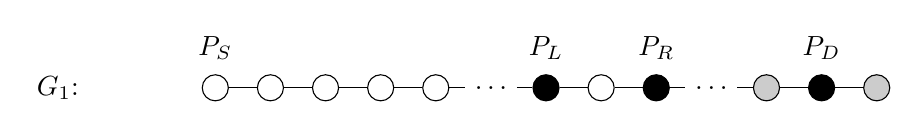
\begin{tikzpicture}[
	edge/.style={-}
	]
	\def\dist{0.7}
	\node at (-2,0) {$G_1$:};
	
	\node[circle,draw] (v1) at (0,0) {}; \node at (0,0.5) {$P_S$}; %{$P_1$}; 
	\node[circle,draw] (v2) at (\dist,0) {};
	\node[circle,draw] (v3) at (2*\dist,0) {}; 
	\node[circle,draw] (v4) at (3*\dist,0) {}; 
	\node[circle,draw] (v5) at (4*\dist,0) {}; 
	\node[] (v6) at (5*\dist,0) {$\dots$};
	\node[circle,draw,fill=black] (v7) at (6*\dist,0) {}; \node at (6*\dist,0.5) {$P_L$};%{$P_{\frac{n}{2}-1}$}; 
	\node[circle,draw] (v8) at (7*\dist,0) {};
	\node[circle,draw, fill=black] (v9) at (8*\dist,0) {}; \node at (8*\dist,0.5) {$P_R$};%{$P_{\frac{n}{2}+1}$}; 
	\node[] (v10) at (9*\dist,0) {$\dots$};
	\node[circle,draw,fill=black!20] (v11) at (10*\dist,0) {}; \node at (10*\dist,0.5) {};%{$P_3$}; 
	\node[circle,draw,fill=black] (v12) at (11*\dist,0) {}; \node at (11*\dist,0.5) {$P_D$}; %{$P_4$}; 
	\node[circle,draw,fill=black!20] (v13) at (12*\dist,0) {}; \node at (12*\dist,0.5) {};%{$P_5$};
	
	\draw[edge] (v1) -- (v2) -- (v3) -- (v4) -- (v5) -- (v6) -- (v7) -- (v8) -- (v9)
	-- (v10) -- (v11) -- (v12) -- (v13);
	\end{tikzpicture}
	\caption{Graphs used to prove the impossibility of THC with adversarial delays. 
		$P_S$ is the sender.
		The corrupted parties (black dots) are: $P_L$ and $P_R$ (they delay messages), and the detective $P_D$. The adversary determines whether $P_D$ (and its two neighbors) are on the left or on the right.}
	\label{fig:imp}
\end{figure}



\subsubsection{Adversarially-Controlled Delay Indistinguishability-based Security Definition}
Before proving the impossibility result, we first formally define our model. This model is as weak as possible while still assuming delays are somewhat controlled by the adversary. We will assume a minimum delay along edges: it takes at least one clock-tick for a message to get from one party to another.

\paragraph{Time and Clocks.}
Many asynchronous or semi-synchronous settings require defining a clock (or clocks) for the parties to use. This is to model the time passing in the real-world so that parties can adapt when messages are not delivered in time, etc. For this impossibility result, however, we only need the adversary to be able to keep track of the time passed. So, when the protocol starts, the adversary only needs to count `ticks,' the smallest unit of time that, say, a global clock would use. This way, it does not matter what other clock functionalities are present in the protocol's model, the adversary ignores it to mount its attack.

For notation, the adversary will mark the time passed by $\tau$.

\paragraph{Delay Algorithms}
In order to give the adversary as little power as possible, we define a public (and arbitrary) randomized algorithm that outputs the delays for a graph for protocol $\Pi$. Both the adversary and challenger have access to this algorithm and can sample from it.

\newcommand{\delayAlg}{\mathsf{DelayAlgorithm}}
\begin{definition}
	A \emph{indistinguishability-delay algorithm (IDA)} for a protocol $\Pi$, $\mathsf{Delay}$\-$\mathsf{Algorithm}_{\Pi}$, is a probabilistic polynomial-time algorithm that takes as input an arbitrary graph outputs unbounded polynomial delays for every time $\tau$ and every edge in the graph. Explicitly, for any graph $G = (V, E)$, $\delayAlg(G)$ outputs $\cT$ such that for every edge $(i,j) \in E_b$ and time $\tau$, $\cT((i,j), \tau) = d_{(i,j), \tau}$ is a delay that is at least one.
\end{definition}

\paragraph{The Indistinguishability Game}
This indistinguishability definition is a game between an adversary $\cA$ and challenger $\cC$ adapted from \cite{MOR15}. Let $\delayAlg$ be an IDA as defined above.
\begin{itemize}
	\item Setup: Let $\cG$ be a class of graphs and $\Pi$ a topology-hiding broadcast protocol that works on any of the networks described by $\cG$ according to our adversarial delay model, and let $\delayAlg$ be a public, fixed IDA algorithm. Without loss of generality, let $\party_1$ have input $x \in \{0,1\}$, the broadcast bit.
	\item $\cA$ chooses two graphs $G_0 = (V_0, E_0)$ and $G_1 = (V_1, E_1)$ from $\cG$ and then a subset $\CS$ of the parties to corrupt. $\CS$ must look locally the same in both $G_0$ and $G_1$. Formally, $\CS \subset V_0 \cap V_1$ and $\nbhi{0}{\CS} = \nbhi{1}{\CS}$. If this doesn't hold, $\cC$ wins automatically.\\
	$\cA$ then generates $\cT_{\CS}$, a function defining delays for every edge at every time-step controlled by the adversary. That is, $\cT_{\CS}((i,j), \tau) = d_{(i,j),\tau}$, and if $\party_i \in \CS$, then every message sent from $\party_i$ to $\party_j$ at time $\tau$ is delayed by an extra $d_{(i,j), \tau}$.\\
	$\cA$ sends $G_0, G_1, \CS,$ and $\cT_{\CS}$ to $\cC$.
	
	\item $\cC$ chooses a random $b \in \{0,1\}$ and executes $\Pi$ in $G_b$ with delays according to $\delayAlg(G_b) = \cT$ for all messages sent from honest parties. For messages sent from corrupt parties, delay is determined by the time and parties as follows: for time $\tau$ a message sent from party $\party_i \in \CS$ to $\party_j$ has delay $\cT((i,j), \tau) + \cT_{\CS}((i,j), \tau)$ in reaching $\party_j$. $\cA$ receives the view of all parties in $\CS$ during the execution.
	
	\item $\cA$ then outputs $b' \in \{0,1\}$ and wins if $b' = b$ and loses otherwise.
\end{itemize}

Notice that in this model, the adversary statically and passively corrupts any set of parties, and statically determines what delays to add to the protocol.

\begin{definition}
	A protocol $\Pi$ is \emph{indistinguishable under chosen delay attack (IND-CDA)} over a class of graphs $\cG$ if for any PPT adversary $\cA$, there exists an IDA $\delayAlg$ such that
	\[ \Pr[\cA \mbox{ wins}]  \leq \frac 1 2 + \negl(n). \]
\end{definition}

\subsubsection{Proof that Adversarially-Controlled Delays Leak Topology}
First, we will define what we mean when we say a protocol is `weakly' realized in the adversarial delay model. Intuitively, it is just that the protocol outputs the correct bit to all parties if there is no adversarial delay.

\begin{definition}
	A protocol $\Pi$ \emph{weakly realizes the broadcast functionality} if $\Pi$ is such that when all parties execute honestly with delays determined by any IDA, all parties get the broadcast bit within polynomial time (with all but negligible probability).
\end{definition}


\begin{theorem}\label{thm:impossibility}
	There does not exist an IND-CDA secure protocol $\Pi$ that weakly realizes the broadcast functionality of any class of graphs $\cG$ that contains line graphs.
\end{theorem}

Throughout the proof and associated claim, we refer to a specific pair of graphs that the adversary has chosen to distinguish between, winning the IND-CDA game. Both graphs will be a line of $n$ vertices: $G = (V,E)$ where $E = \{(\party_i, \party_{i+1})\}_{i=1,\ldots,n-1}$. We will let $\Pi$ be a protocol executed on $G$ that weakly realizes broadcast when $P_1$ is the broadcaster, see Figure \ref{fig:imp}.

Our adversary in this model will either add no delay, or will add a very long polynomial delay to every message sent after some time $\tau$.

Notice that $\cA$ is given access to $\delayAlg$ at the start of the protocol. One can sample from $\delayAlg$ using $G_0$, $G_1$, and $\CS$ to get an upper bound $T$ on the time it takes $\Pi$ to terminate with all but negligible probability. Since $\Pi$ weakly realizes broadcast, $T$ is polynomial. So, $\cA$ has access to this upper bound $T$.


\paragraph{Long-delays.} Let a long-delay be a delay that lasts for $T$ clock-ticks. Consider an adversary that will only add long-delays to a protocol, and once an adversary has long-delayed a message, he must continue to long-delay messages along that edge until the end of the protocol. That is, once the adverary decides to delay along some edge, all subsequent messages along that edge cannot arrive for at least $T$ clock-ticks.

\begin{claim}
	Consider any party $\party_v$ whose neighbors do not add any extra delay as described by the long-delay paragraph above. As in \cite{MOR15}, let $H_{v,b}$ be the event that $\party_v$ outputs the broadcast bit by time $T$ ($\party_v$ may still be running the protocol by time $T$ or terminate by guessing a bit by $T$). 
	Let $E_\tau$ be the event that the first long-delay is at time $\tau$. Then either $\Pi$ is not IND-CDA secure, or there exists a bit $b$ such that 
	\[ \lvert \Pr \left[ H_{v,b} | E_{T-1} \right] - \Pr \left[ H_{v,b} | E_{0} \right] \rvert \geq \frac 1 2 - \negl(n).\]
\end{claim}
\begin{proof}
	If some $\party_i$ long-delays at time $0$, then the first message it sends is at time $T$, and so the graph is disconnected until time $T$. This makes it impossible for parties separated from $\party_1$ to learn about the output bit by time $T$. So, by that time, these parties must either guess an output bit (and be right with probability at most 1/2) or output nothing and keep running the protocol (which is still not $H_{v,b}$). If $\Pi$ is IND-CDA secure, then all honest parties must have the same probability of outputting the output bit by time $T$, and so there exists a $b$ such that $\Pr[H_{v,b} | E_0] \leq \frac 1 2 - \negl(n)$ for all honest parties $\party_v$.
	
	However, if $\party_i$ long-delays at time $T-1$, then the only parties possibly affected by $\party_i$ are $\party_{i-1}$ and $\party_{i+1}$; all other parties will get the output by time $T$ and the information that $\party_i$ delayed cannot reach them (recall we assumed a minimum delay of at least one clock-tick in the $\delayAlg$). So, $\Pr[H_{v,b} | E_0] = \Pr[H_{v,b} | \mbox{no extra delays}] = 1 - \negl(n)$ for all honest parties without a delaying neighbor by the definition of weakly realizing broadcast.
	
	The claim follows: $\lvert \Pr \left[ H_{v,b} | E_{T-1} \right] - \Pr \left[ H_{v,b} | E_{0} \right] \rvert \geq \lvert \frac 1 2 - \negl(n) - 1 
	\rvert \geq \frac 1 2 - \negl(n)$.
	\qed
\end{proof}

\begin{proof}[Theorem \ref{thm:impossibility}]
	This just follows from the previous claim. A simple hybrid argument shows that there exists a pair $(\tau^*, b) \in \{0,\ldots, T-1\} \times \{0,1\}$ such that 
	\[ \lvert \Pr \left[H_{v,b} | E_{\tau^*} \right] - \Pr \left[ H_{v,b} | E_{\tau^* + 1} \right] \rvert \geq \frac 1 {2T} - \negl(n) \]
	for all $P_v$ who do not have a neighbor delaying. Since $T$ is polynomial, this is a non-negligible value. Without loss of generality, assume $\Pr[ H_{v,b} | E_{\tau^*}] > \Pr[H_{v,b} | E_{\tau^* + 1}]$. Leveraging this difference, we will construct an adversary $\cA$ that can win the IND-CDA game with non-negligible probability.
	
	$\cA$ chooses two graphs $G_0$ and $G_1$. $G = G_0$ and $G_1$ is $G$ except parties 3, 4, and 5 are exchanged with parties $n-2$, $n-1$, and $n$ respectively. $\cA$ corrupts the source part $\party_S := \party_1$, a left party $\party_L := \party_{n/2-1}$, a right party $\party_R := \party_{n/2 + 1}$, and the detective party $\party_D := \party_4$. See figure \ref{fig:imp} for how this looks. The goal of $\cA$ will be to determine if $\party_D$ is to the left or right side of the network (close to the broadcaster or far).
	
	$\cA$ computes the upper bound $T$ using $\delayAlg$ and randomly guesses $(\tau^*, b)$ that satisfy the inequality above. At time $\tau$, $\cA$ initiates a long-delay at party $\party_L$, and at time $\tau+1$, $\cA$ initiates a long-delay at party $\party_R$. So, $\cA$ gives the challenger $\cT_{\CS}$ where $\cT_{\CS}((i,j), t) = 0$ for $t < \tau^*$, and for $t \geq \tau^*$: $\cT_{\CS}((L, n/2), t) = \cT_{\CS}((L, n/2-2), t) T$ and $\cT_{\CS}((R, n/2), t+1) = \cT_{\CS}((R, n/2 + 2), t+1) = T$.
	
	Notice that news of $P_L$'s delay at time $\tau^*$ cannot reach $P_R$ or any other party on the right side of the graph by time $T$. Also note that the time $\cA$ gets output for each of its corrupt parties is noted in the trasncript.
	
	If $\cC$ chooses $G_0$, then $\party_D$ is on the left side of the graph and has probability $\Pr[H_{D, b} | E_{\tau^*}]$ of having the output bit by time $T$ because its view is consistent with $\party_L$ delaying at time $\tau^*$.
	If $\cC$ chooses $G_1$, then $\party_D$ is on the right side of the graph, and has a view consistent with the first long delay happening at time $\tau^*+1$ and therefore has $\Pr[H_{D,b} | E_{\tau^*}]$ of having the output bit by time $T$.
	Because there is a noticeable difference in these probabilities, $\cA$ can distinguish between these two cases with $\frac 1 2$ plus some non-negligible probability.
\end{proof}

\paragraph{Consequences of this lower bound.}
We note that this is just one model where we prove it is impossible for the adversary to control delays. However, we restrict the adversary a great deal, to the point of saying that regardless of what the natural network delays are, the adversary can learn something about the topology of the graph. The lower bound proved in this model seems to rule out any possible model (simulation or game-based) where the adversary has power over delays.







